\chapter{Conclusions and Future Work}\label{ch:conclusions}

This thesis presents a \acrshort{dt} for smart homes that can forecast and optimize the energy consumption of various appliances in a smart home. A hypothetical home was used as a case study to design and test the \acrshort{dt}, since no real home was available. The hypothetical home included a range of appliances that were representative of typical smart home scenarios.

A scoping review of existing smart home datasets was performed to select suitable data sources for the appliances. The review revealed that power consumption datasets were the most relevant and available, but none of them contained information about the operation modes of the appliances. To address this limitation, 15 appliances from the GREEND and UK-DALE datasets were chosen, and their operation modes were inferred using a hybrid \acrshort{ml} method and the manufacturers' manuals.

The \acrshort{dt} was implemented as a \acrshort{rest} \acrshort{api}, which offers several endpoints to access and manipulate information about appliances, routines, and consumptions. The \acrshort{api} also allows to simulate the addition of new routines and provides feedback and suggestions to improve energy efficiency. A frontend application was developed to showcase the functionality and usability of the \acrshort{dt}.

\paragraph{Physical Twin}

The \acrshort{dt} developed in this thesis is a digital-only system that cannot interact with the physical world directly. To enable this interaction, it needs to connect to the smart devices in the home and send commands to them. This entails developing a physical twin similar to the hypothetical home presented in Chapter~\ref{ch:hypothetical_home}. The \acrshort{dt} should also update the state of the devices and the energy consumption according to the changes in the physical world.

\paragraph{Appliance Data}

Future versions of the \acrshort{dt} should let users add new appliances by automatically importing their consumption values and operation modes. This requires having a list of smart devices that are compatible with the \acrshort{dt}, and whose data are accessible during the system configuration. Since the appliance data format is custom, it may be necessary to use a standardized format for the data or develop a system that can automatically convert the data from the appliance to the format used by the \acrshort{dt}.

These consumption values should be treated as approximate and based on the new and optimal functioning of the appliance. Over time, the \acrshort{dt} should learn from the actual consumption, as they may vary due to malfunctions or lack of maintenance.

The \acrshort{dt} could also work with non-smart appliances that do not provide information about themselves, by using a \acrshort{ml} approach similar to the one used in Chapter~\ref{ch:hypothetical_home} to automatically detect the operation modes and consumptions.

\paragraph{Manual Appliance Activation}

The \acrshort{dt} should be able to handle the manual activation of appliances by end users, by automatically detecting their state changes and resolving conflict C3 (see Section~\ref{sec:simulation}).

Moreover, the \acrshort{dt} could monitor the manual activations of appliances and their duration, and use this information to provide suitable recommendations to automate the activations or modify existing routines. For instance, if the user starts the computer every day at 9:00, the \acrshort{dt} could propose to automate this activation. If the computer stays on for 8 hours on average, the \acrshort{dt} can use this information to anticipate whether this could cause any conflict with existing routines, and avoid them before they occur.

\paragraph{Predictions over Multiple Days}

Currently, the \acrshort{dt} can only predict the energy consumption for the current day. Future versions should enable the system to predict the energy consumption for several days ahead, and also view the consumption history for the previous days. This would allow the system to provide more precise recommendations, and to better handle the conflicts between routines. For example, if the user is planning to go on vacation for a week, the \acrshort{dt} could advise to turn off the heating system, and to turn off the refrigerator for the vacation period.

\paragraph{Authentication}

Future developments should implement an authentication scheme to secure the \acrshort{dt} from unauthorized access. This would enable the system to be used in a multi-user environment, where users may have different roles and permissions. This could be beneficial for a family, where the children are restricted from changing routines, and have limited access to creating new ones. For instance, they may be prohibited from creating routines that involve the dishwasher or the washing machine, and they may only activate the TV for a certain amount of time. The parents, on the other hand, may have full access to the system and could also monitor the children's activities.

\paragraph{Frontend}

To allow the end users to interact with the \acrshort{dt} effectively and also consider the future developments mentioned in the previous sections, a more comprehensive frontend application than the showcase one developed in this thesis is required. A frontend application for Android devices that meets these requirements is currently being developed as part of the broader research project.

\vspace*{\fill} % Spazio bianco per mettere il testo in fondo alla pagina

\begin{figure}[h]
    \centering
    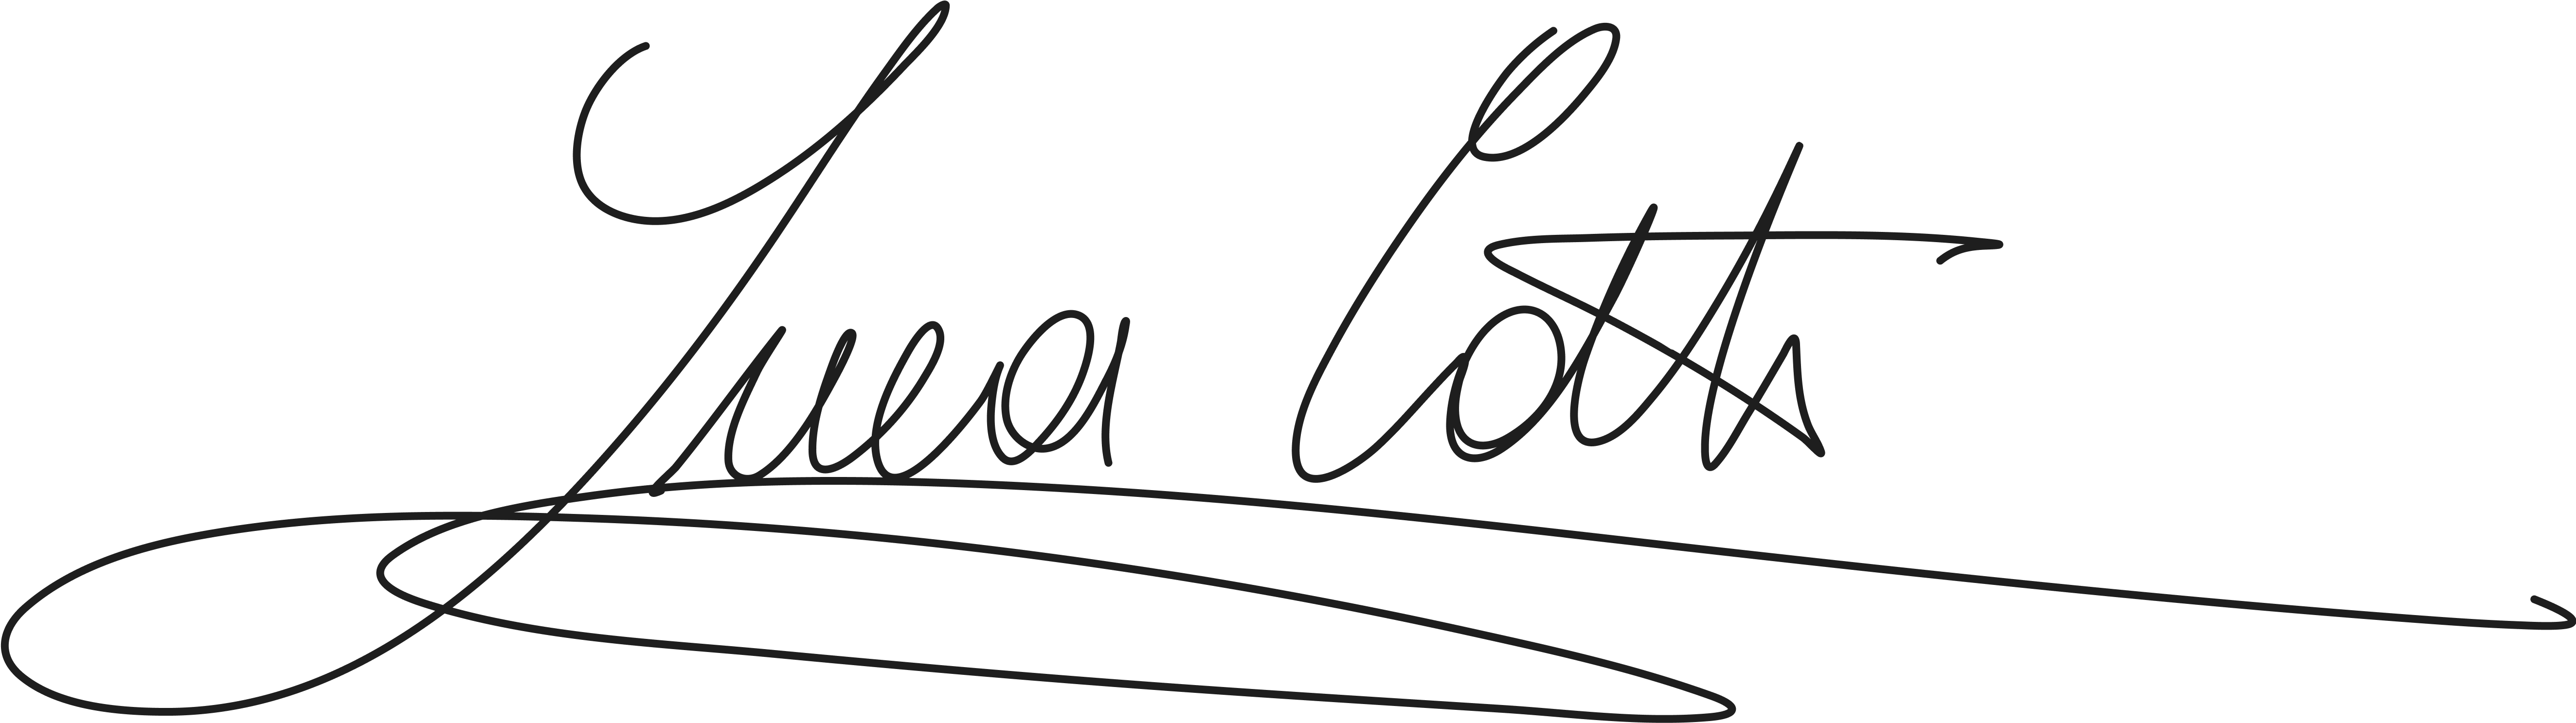
\includegraphics[width=.7\textwidth]{images/signature.png}
\end{figure}

\vspace*{16mm} % Spazio bianco per mettere il testo in fondo alla pagina